\documentclass[aps,pre,twocolumn,superscriptaddress,nofootinbib,floatfix]{revtex4-2}

\usepackage[utf8]{inputenc}
\usepackage[T1]{fontenc}
\usepackage{lmodern}
\usepackage[brazil]{babel}
\usepackage{graphicx}
\usepackage{amsmath,amssymb}
\usepackage{bm}
\usepackage{siunitx}
\sisetup{output-decimal-marker={,}}
\usepackage{booktabs}
\usepackage{subcaption}
\usepackage[hidelinks]{hyperref}

\graphicspath{{figures/}}
\newcommand{\mac}[1]{\left\langle #1 \right\rangle}

\raggedbottom
\begin{document}

\renewcommand{\figurename}{Fig.}
\renewcommand{\tablename}{Tabela}

\title{O canhão de réguas: armazenamento de energia elástica e liberação\\ limitada por atrito de um projétil comprimido entre duas réguas}

\author{Gabriel Bassi}
\affiliation{Equipe Brasil, International Young Physicists' Tournament (IYPT) 2025}

\begin{abstract}
Quando um projétil redondo é comprimido entre duas réguas presas uma à outra em uma extremidade, uma força adicional aplicada sobre as réguas pode ejetá-lo em alta velocidade. Explicamos o efeito como a liberação, limitada por atrito, da energia elástica armazenada nas réguas fletidas: o projétil é retido pelo atrito estático até que a força adicional aumente a inclinação das réguas no ponto de contato além do ângulo de atrito. Modelando cada régua como uma viga em balanço de Euler--Bernoulli, formulada com colchetes de Macaulay e verificada pelo teorema de Castigliano, obtemos a matriz de flexibilidade do sistema, que é simétrica pela reciprocidade de Maxwell--Betti, a força de contato e a força adicional necessária ao lançamento. Esta última define uma \emph{zona de retenção} $x_0>3r/2\mu_s$, fora da qual o projétil é ejetado espontaneamente, e é mínima quando o atuador está a dois terços da distância entre o engaste e o projétil. Escrevendo o balanço de energia como o trabalho das forças de contato ao longo das réguas, incluindo o atrito cinético, o atrito dos discos com a base e a inércia das réguas, obtemos a velocidade de ejeção em forma fechada no limite de pequenas inclinações, com $v\propto\sqrt{EI}$. Experimentos com um lançador motorizado e reprodutível e um sensor de velocidade por barreiras de laser, usando esferas e discos impressos em 3D de raio e massa controlados, mostram as tendências previstas: a velocidade diminui com o raio, a posição inicial e a massa do projétil e aumenta com a distância da força adicional. Uma única família de réguas, porém, não reproduz as velocidades absolutas das quatro séries de medidas.
\end{abstract}

\maketitle

%=====================================================================
\section{Introdução}
\label{sec:intro}
%=====================================================================

O International Young Physicists' Tournament (IYPT) de 2025 propôs o seguinte problema~\cite{iypt2025}:
\begin{quote}
\emph{Duas réguas são mantidas firmemente uma contra a outra. Um projétil redondo (por exemplo, uma tampa de garrafa plástica ou uma bola) é inserido entre elas, próximo a uma de suas extremidades. Quando uma força extra é exercida sobre a superfície das réguas, o projétil é ejetado em alta velocidade. Investigue esse efeito e os parâmetros que afetam a velocidade de ejeção.}
\end{quote}
O dispositivo é um lançador elástico simples, no qual a energia é armazenada na flexão de duas vigas esbeltas e liberada através de um contato com atrito. Sua análise combina a teoria clássica de vigas~\cite{timoshenko1972,gere2009}, métodos de energia~\cite{castigliano} e o atrito estático e cinético. Neste artigo descrevemos o mecanismo qualitativamente (Sec.~\ref{sec:qualitative}), apresentamos um arranjo experimental reprodutível (Sec.~\ref{sec:setup}), desenvolvemos um modelo quantitativo (Sec.~\ref{sec:theory}) e comparamos suas previsões com medidas da velocidade de ejeção em função do raio, da massa e da posição do projétil e da posição da força aplicada (Sec.~\ref{sec:results}).

%=====================================================================
\section{Descrição qualitativa}
\label{sec:qualitative}
%=====================================================================

O lançamento ocorre em três etapas (Fig.~\ref{fig:phenomenon}). (i)~A inserção da bola entre as réguas as afasta; a força elástica restauradora pressiona a bola, e o atrito estático a mantém no lugar. (ii)~Uma força extra é aplicada nas faces externas das réguas. Ela aumenta o momento fletor e, portanto, a inclinação das réguas no ponto de contato, de modo que a componente da força de contato que empurra a bola para fora cresce até exceder o atrito estático máximo. (iii)~A bola então desliza ou rola ao longo das réguas, que se fecham atrás dela, convertendo a energia elástica armazenada em energia cinética do projétil.

\begin{figure}[t]
  \centering
  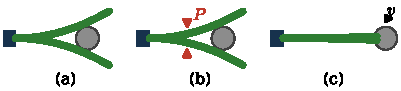
\includegraphics[width=\columnwidth]{stages.pdf}
  \caption{Etapas do lançamento (vista superior; as réguas estão engastadas à esquerda). (a)~A bola deflete as réguas e é retida pelo atrito estático. (b)~Uma força extra $P$ (setas vermelhas) aumenta a flexão e a inclinação das réguas no ponto de contato. (c)~Vencido o atrito estático, as réguas se fecham e a bola é ejetada com velocidade $v$.}
  \label{fig:phenomenon}
\end{figure}

%=====================================================================
\section{Arranjo experimental}
\label{sec:setup}
%=====================================================================

O arranjo (Fig.~\ref{fig:setup}) consiste em uma base de MDF cortada a laser, que mantém as duas réguas engastadas juntas em uma extremidade, dois atuadores lineares impressos em 3D que aplicam a força extra, um sensor de velocidade por barreiras de laser e um conjunto de projéteis impressos em 3D.

\begin{figure}[t]
  \centering
  \begin{subfigure}[b]{0.49\columnwidth}\centering
    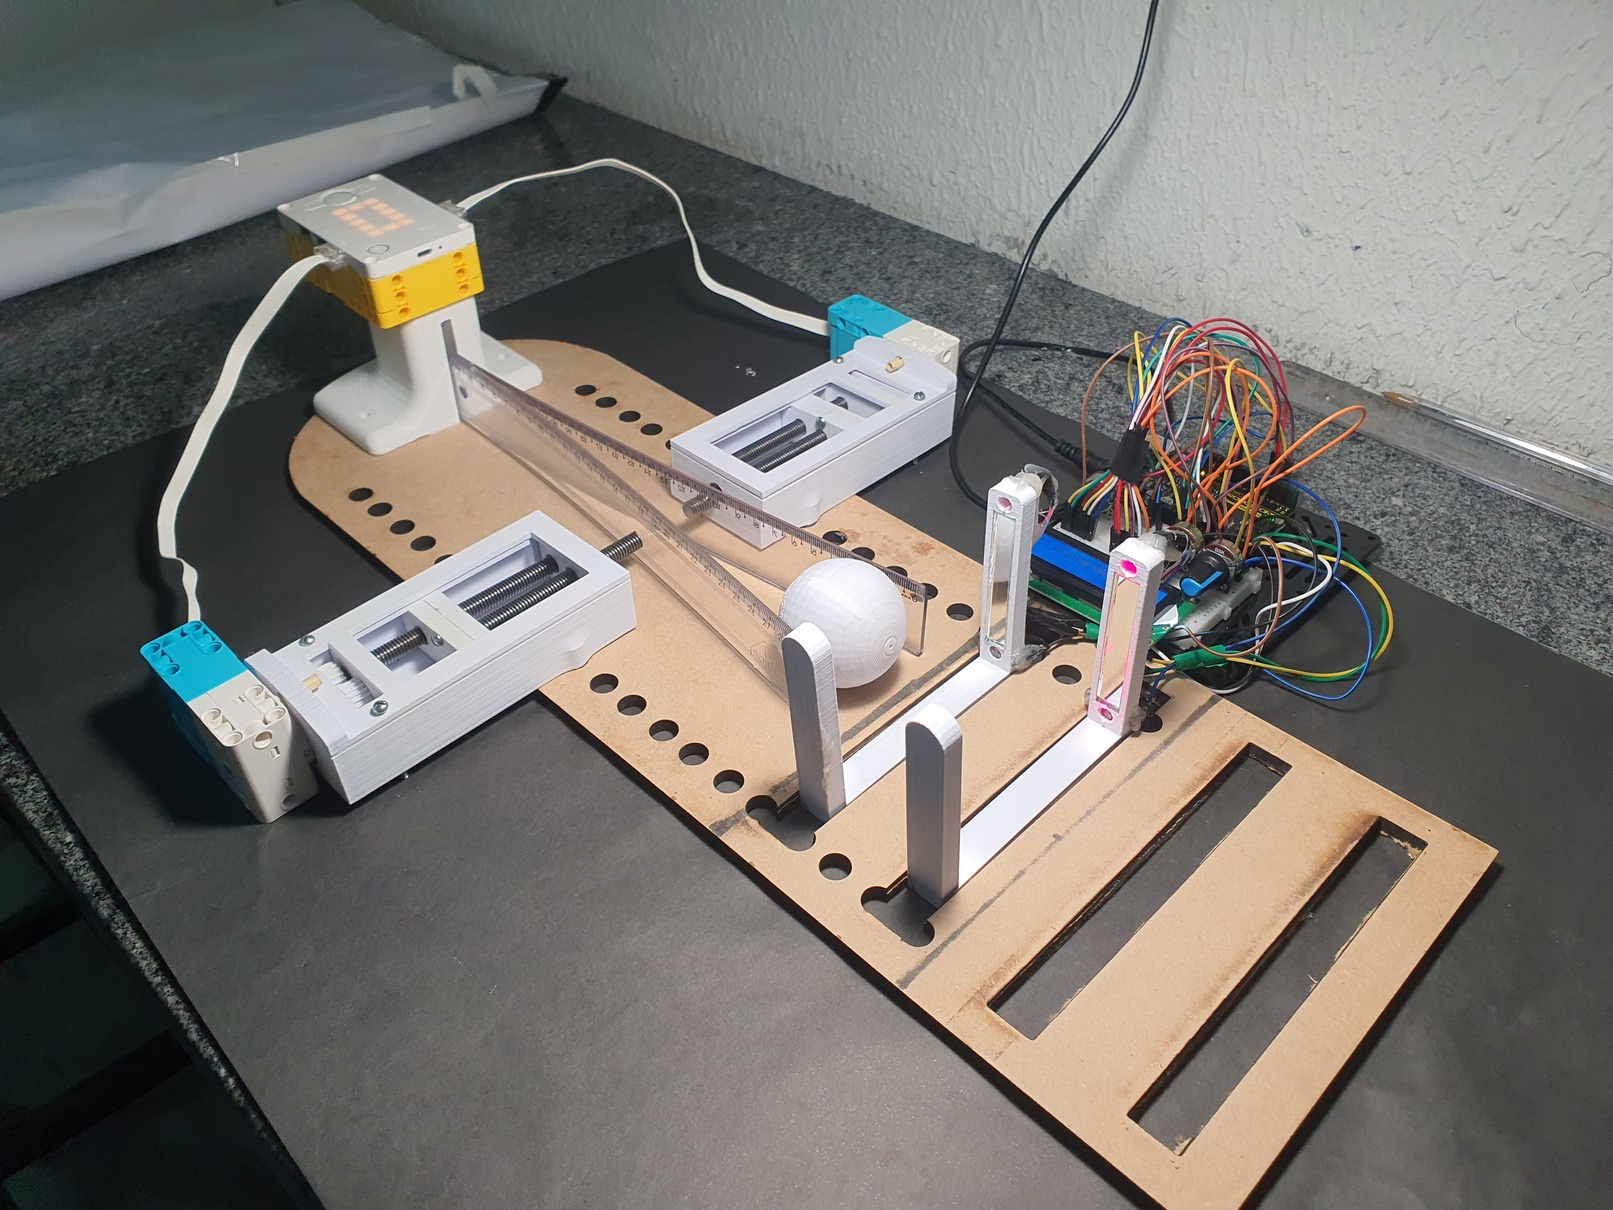
\includegraphics[width=\linewidth]{setup_photo.jpg}\caption{}\end{subfigure}\hfill
  \begin{subfigure}[b]{0.49\columnwidth}\centering
    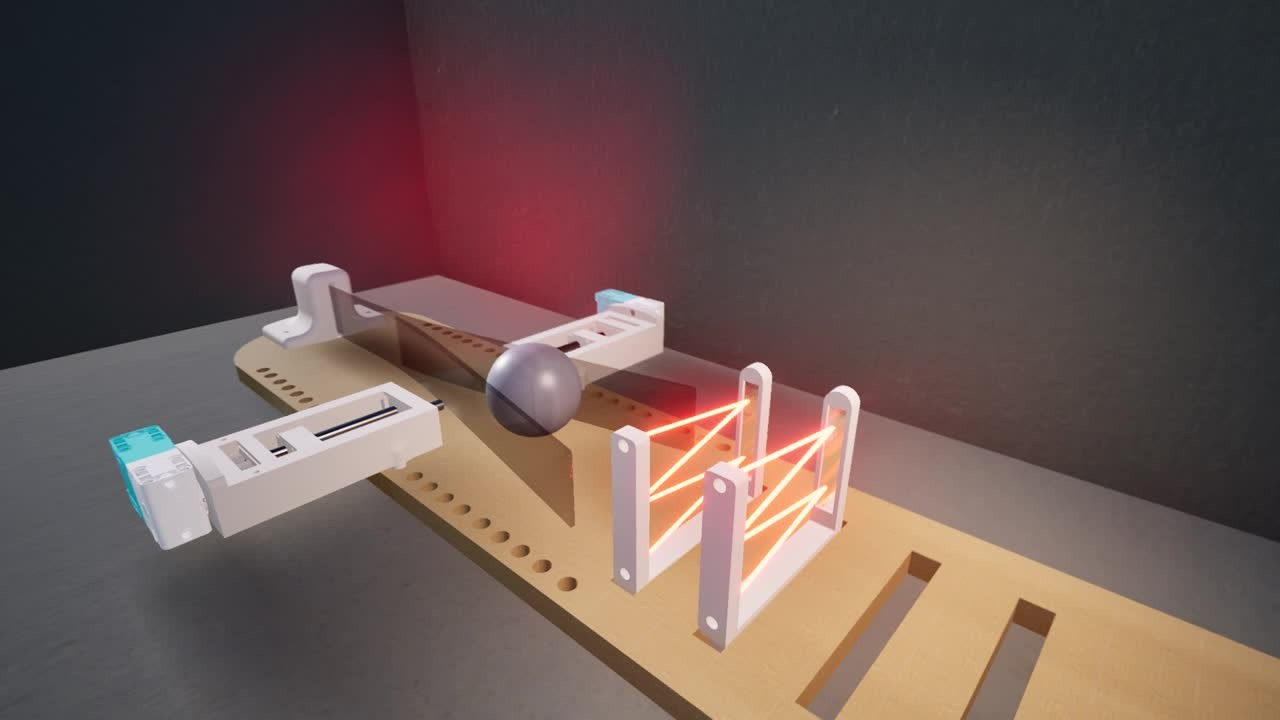
\includegraphics[width=\linewidth]{setup_render.jpg}\caption{}\end{subfigure}
  \caption{(a)~Arranjo experimental: base de MDF, réguas, atuadores lineares, projétil e barreiras de laser. (b)~Modelo CAD do arranjo.}
  \label{fig:setup}
\end{figure}

\paragraph*{Atuadores lineares.} Um atuador linear converte a rotação de um fuso em movimento linear. Dois atuadores, impressos em 3D a partir de nosso próprio projeto CAD e equipados com hastes de aço, pressionam as faces externas das réguas e as defletem ainda mais [Fig.~\ref{fig:sensor}(a)]. Cada um é acionado por um motor LEGO Spike Prime cujo codificador conta as rotações com precisão, e ambos são ativados simultaneamente pelo controlador Spike Prime. A velocidade horizontal das hastes é pequena em comparação com a velocidade com que as réguas retornam, de modo que a força que exercem pode ser considerada constante durante o lançamento.

\paragraph*{Sensor de velocidade.} A velocidade de ejeção é medida com duas barreiras de laser [Fig.~\ref{fig:sensor}(b,c)]. Cada barreira consiste em um emissor laser e um resistor dependente de luz (LDR) ligado a um Arduino. Quando o projétil interrompe o primeiro feixe, um cronômetro é iniciado; quando interrompe o segundo, o intervalo é exibido. A velocidade de ejeção é $v=\Delta s/\Delta t$, onde $\Delta s$ é a separação fixa entre os feixes e $\Delta t$ o tempo de trânsito medido; a incerteza temporal, obtida como o desvio padrão de medidas repetidas, é $\sigma=\SI{0.276}{ms}$. Como as barreiras ficam imediatamente após a extremidade das réguas, $v$ é a velocidade com que o projétil as deixa.

\begin{figure}[t]
  \centering
  \begin{subfigure}[b]{\columnwidth}\centering
    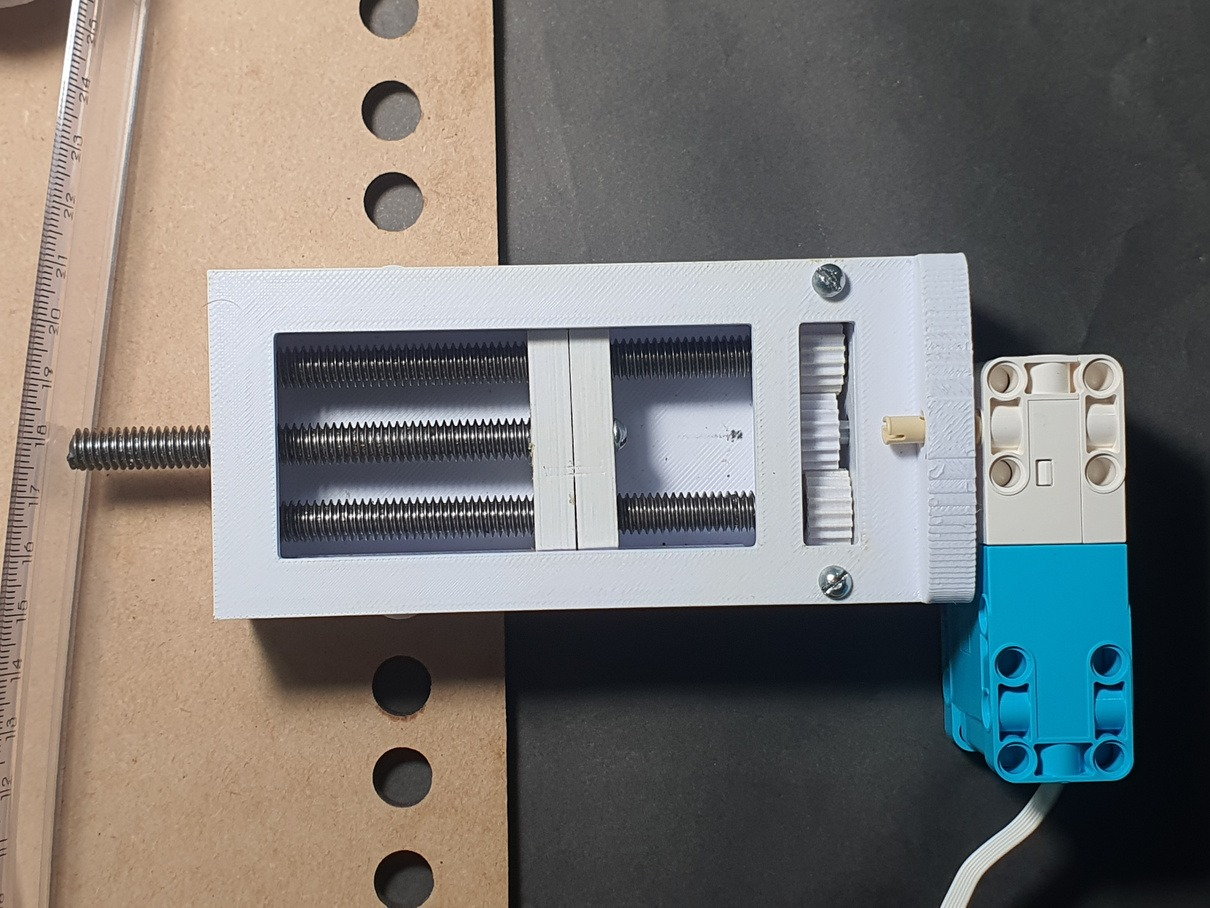
\includegraphics[width=0.7\linewidth]{actuator.jpg}\caption{}\end{subfigure}\\[2pt]
  \begin{subfigure}[b]{0.49\columnwidth}\centering
    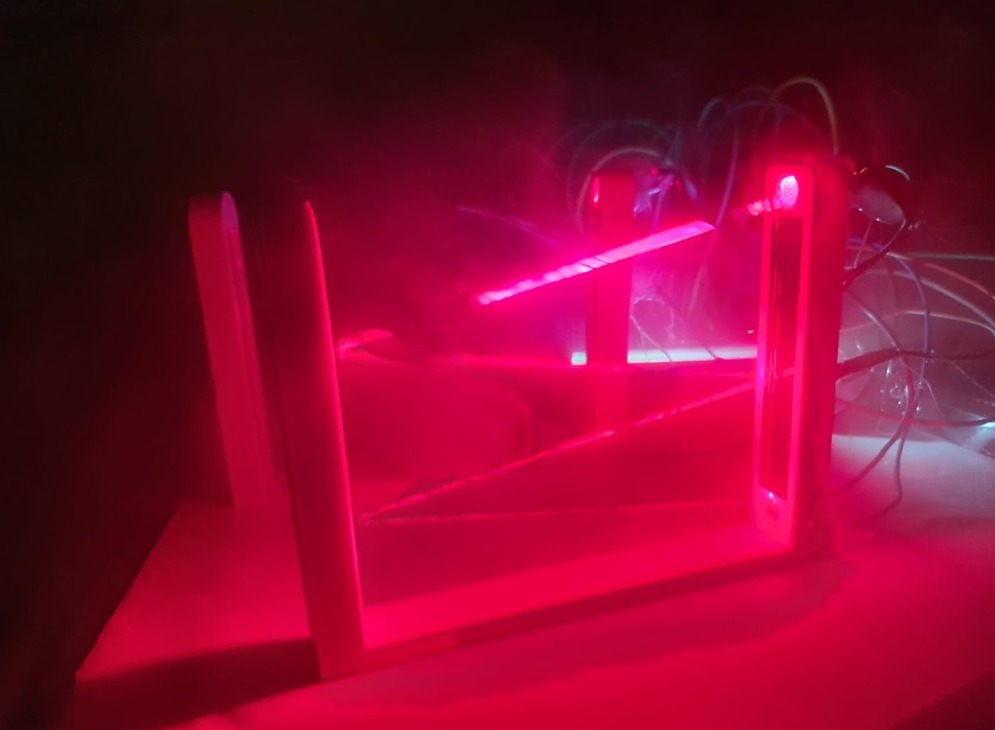
\includegraphics[width=\linewidth]{sensor_lasers.jpg}\caption{}\end{subfigure}\hfill
  \begin{subfigure}[b]{0.49\columnwidth}\centering
    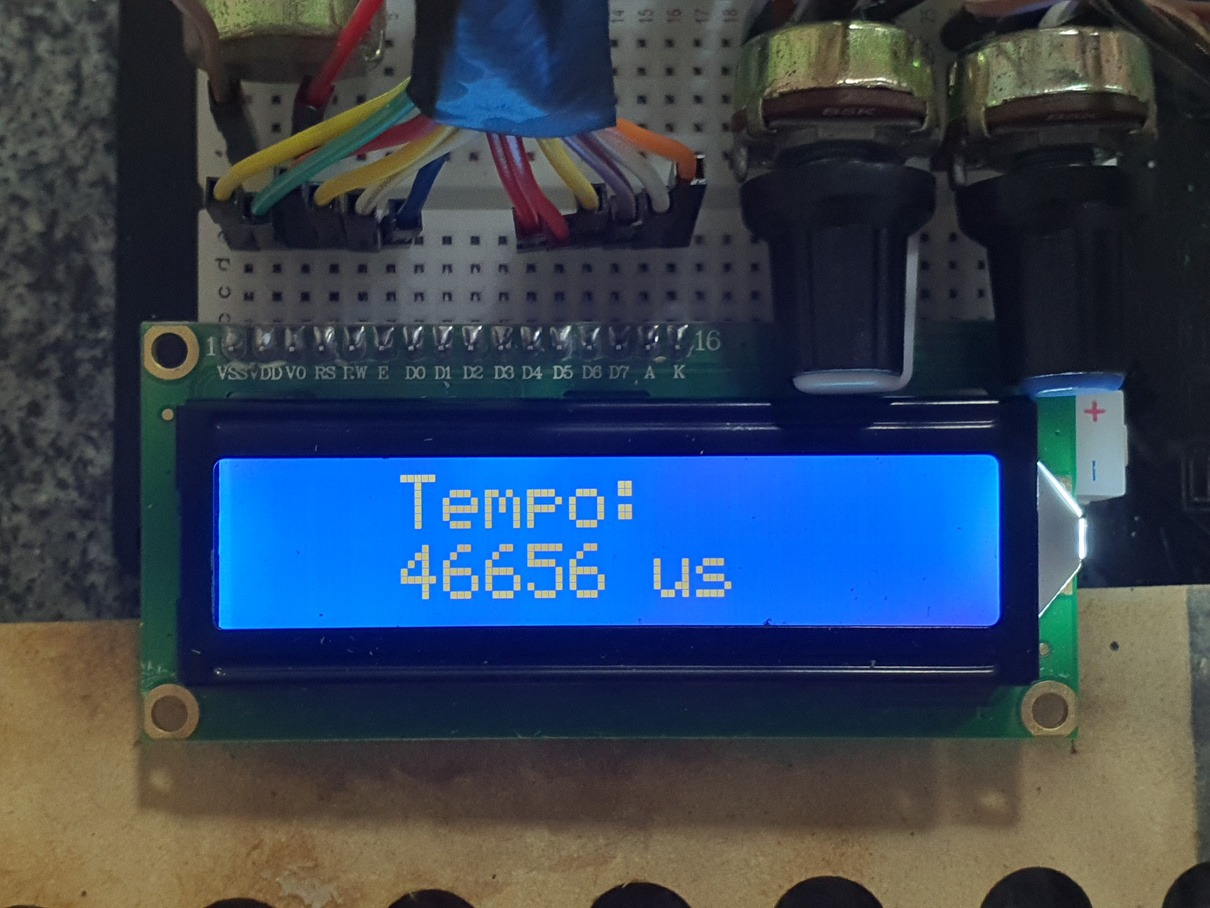
\includegraphics[width=\linewidth]{sensor_display.jpg}\caption{}\end{subfigure}
  \caption{(a)~Atuador linear impresso em 3D, acionado por um motor Spike Prime. (b)~As duas barreiras de laser do sensor de velocidade. (c)~Visor do Arduino mostrando o tempo de trânsito entre as barreiras.}
  \label{fig:sensor}
\end{figure}

\paragraph*{Projéteis.} Esferas e discos cilíndricos foram impressos em 3D (Fig.~\ref{fig:projectiles}). Para variar o raio com massa constante, e a massa com raio constante, ajustou-se a densidade de preenchimento das impressões. As duas séries estão listadas na Tabela~\ref{tab:projectiles}.

\begin{table}[b]
  \caption{Projéteis. Os diâmetros têm incerteza de $\pm\SI{0.05}{cm}$ e as massas de $\pm\SI{0.3}{g}$.}
  \label{tab:projectiles}
  \begin{ruledtabular}
  \begin{tabular}{lcccc}
    \multicolumn{5}{l}{\emph{Série de raio (massa constante)}}\\
    Diâmetro (cm)      & 4,00 & 5,00 & 6,00 & 7,00 \\
    Massa do disco (g) & 28,7 & 28,7 & 28,7 & 28,7 \\
    Massa da esfera (g)& 33,8 & 33,8 & 33,8 & 33,8 \\
    \midrule
    \multicolumn{5}{l}{\emph{Série de massa (diâmetro constante, \SI{4.00}{cm})}}\\
    Massa (g)          & 20,0 & 30,0 & 40,0 & 50,0 \\
  \end{tabular}
  \end{ruledtabular}
\end{table}

\begin{figure}[t]
  \centering
  \begin{subfigure}[b]{0.36\columnwidth}\centering
    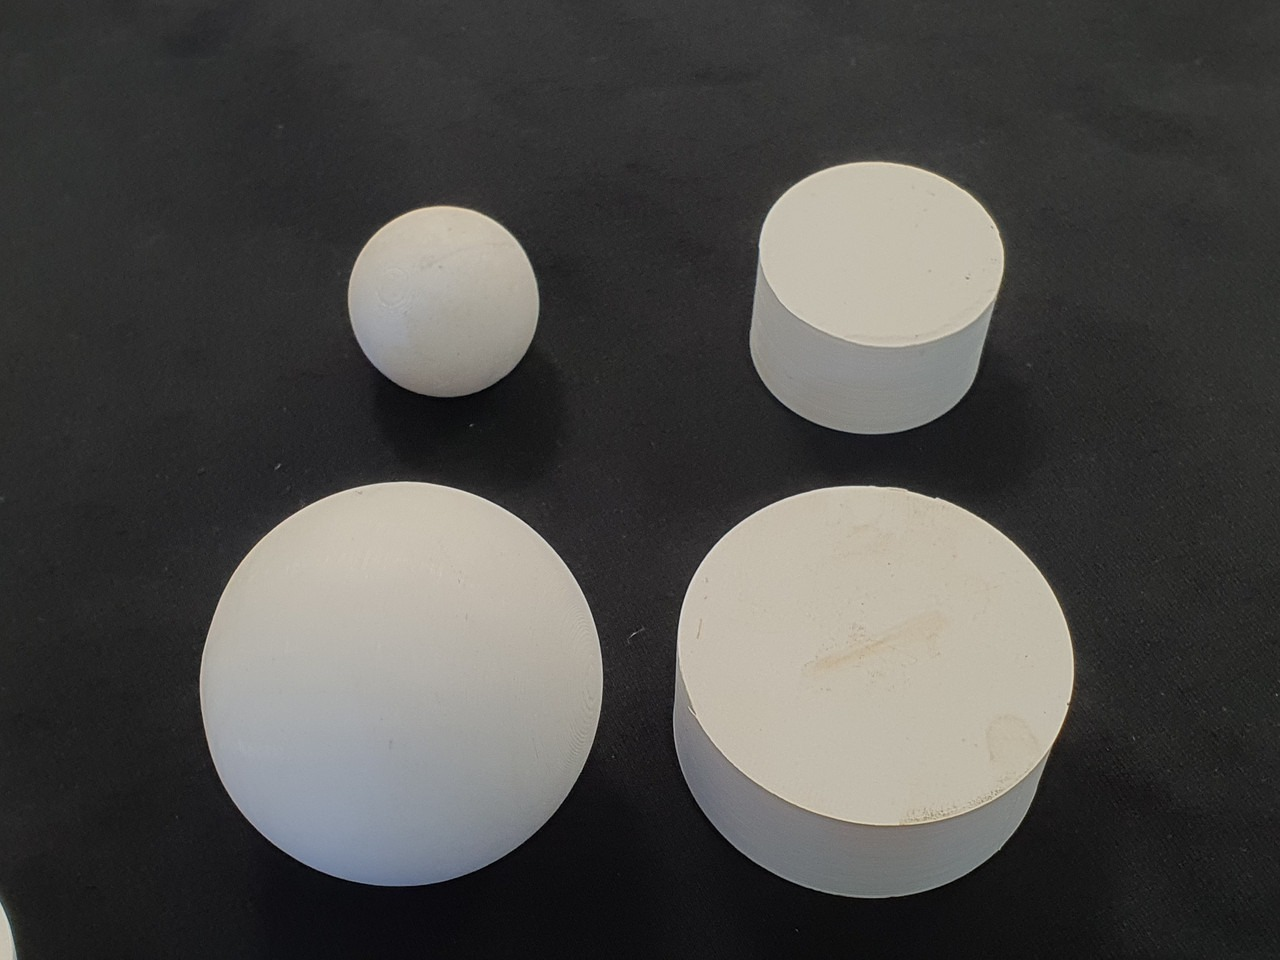
\includegraphics[width=\linewidth]{projectiles.jpg}\caption{}\end{subfigure}\hfill
  \begin{subfigure}[b]{0.26\columnwidth}\centering
    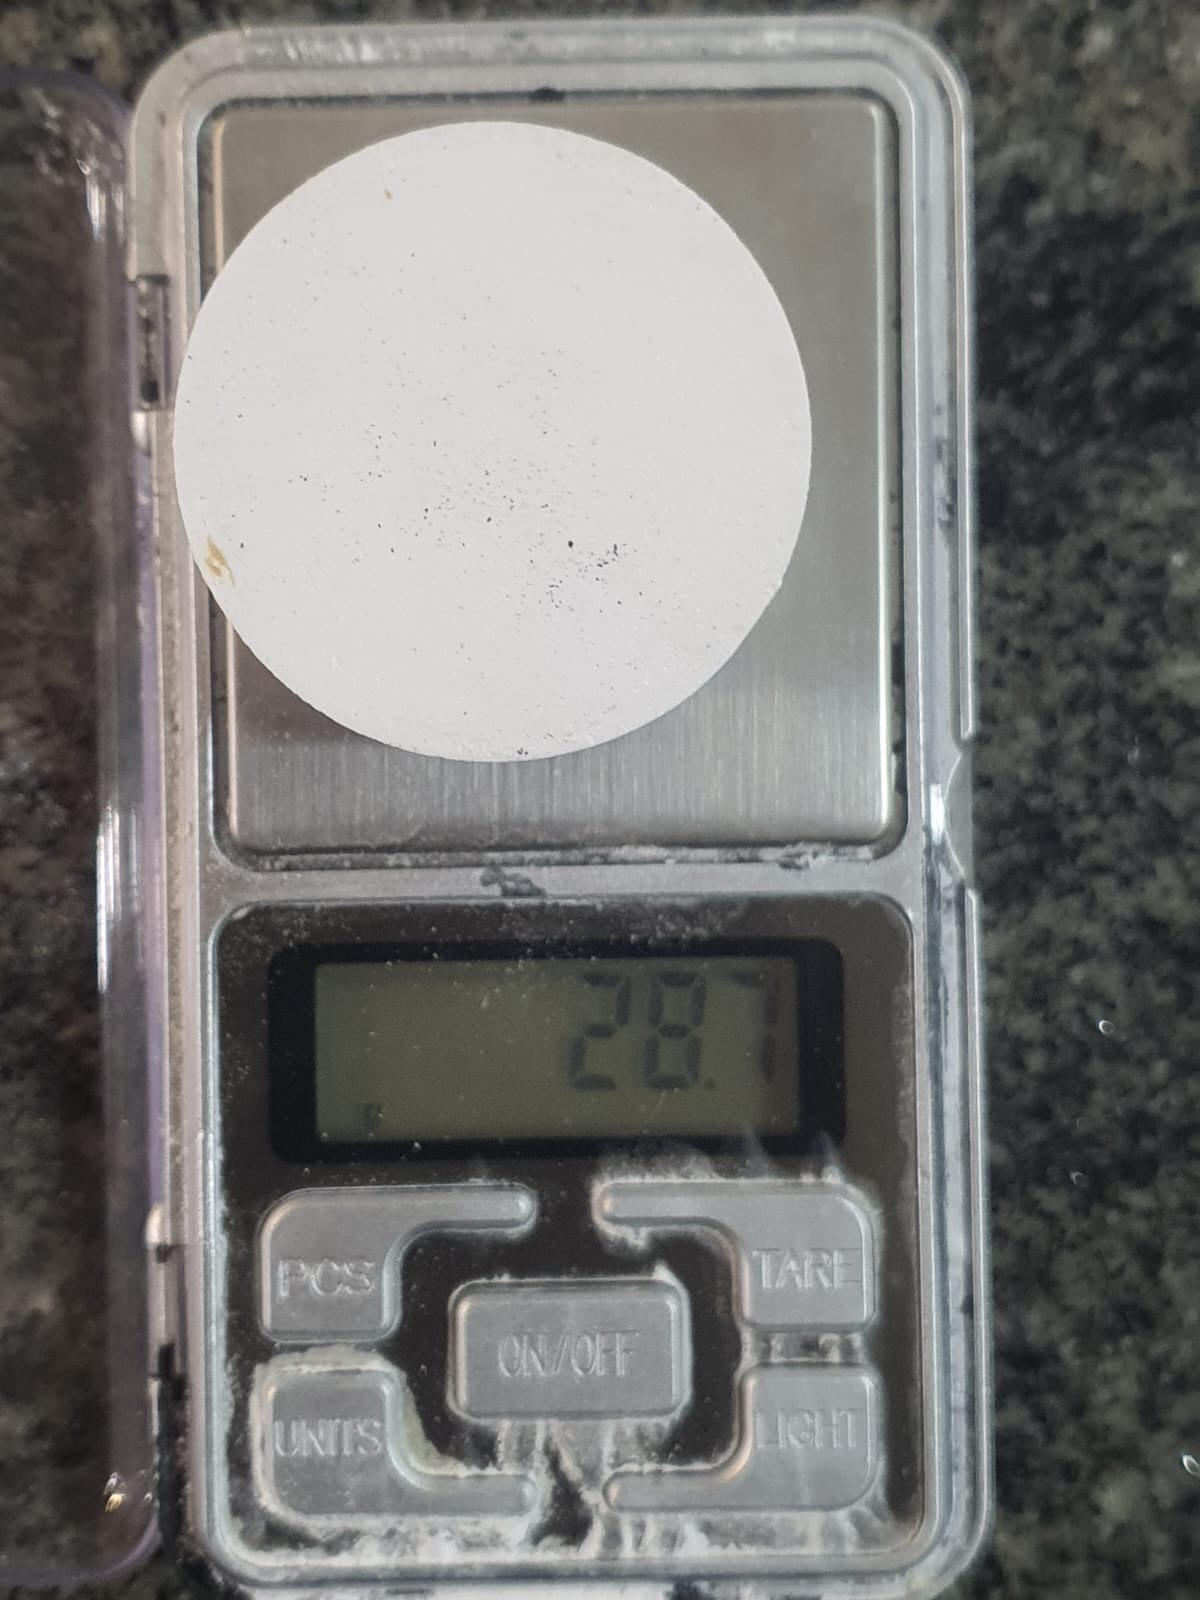
\includegraphics[width=\linewidth]{projectile_mass.jpg}\caption{}\end{subfigure}\hfill
  \begin{subfigure}[b]{0.34\columnwidth}\centering
    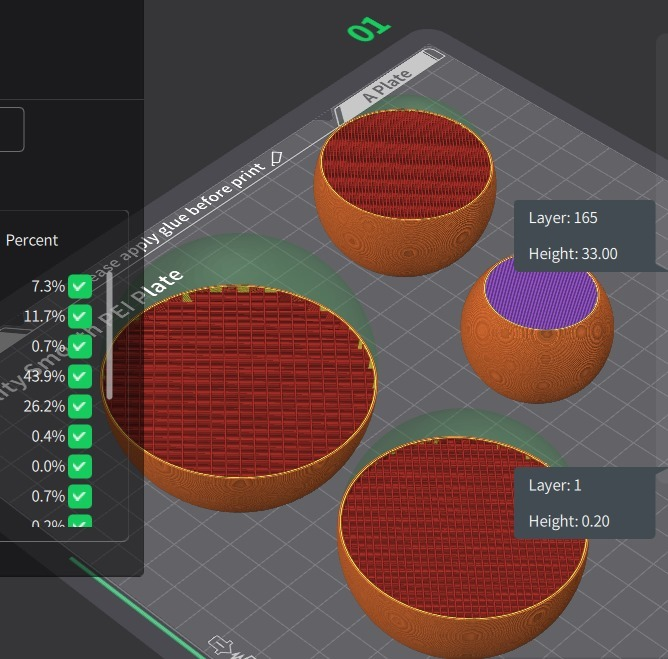
\includegraphics[width=\linewidth]{projectile_infill.jpg}\caption{}\end{subfigure}
  \caption{(a)~Esferas e discos impressos em 3D de diferentes diâmetros. (b)~Verificação da massa em balança de precisão. (c)~Vista do fatiador: a densidade de preenchimento fixa a massa para um diâmetro dado.}
  \label{fig:projectiles}
\end{figure}

\paragraph*{Procedimento.} Para cada valor de parâmetro, o projétil é colocado em sua posição inicial e os atuadores são acionados. Se o lançamento falha, ele é repetido. Cada configuração foi medida três vezes, e as réguas foram substituídas a cada seis lançamentos para limitar o efeito da fadiga (Fig.~\ref{fig:procedure}). Foram usados três tipos de pares de réguas de rigidezes diferentes (réguas~1--3); um par desgastado foi sempre substituído por outro idêntico. No modelo, as réguas entram apenas por sua rigidez à flexão $EI$, por sua massa e por seus coeficientes de atrito com o projétil.

\begin{figure}[t]
  \centering
  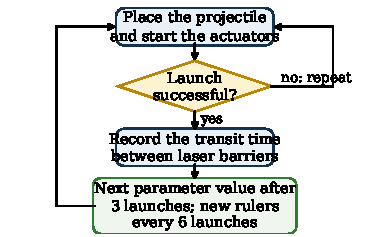
\includegraphics[width=0.9\columnwidth]{procedure.pdf}
  \caption{Procedimento experimental para cada valor de parâmetro.}
  \label{fig:procedure}
\end{figure}

%=====================================================================
\section{Modelo teórico}
\label{sec:theory}
%=====================================================================

\subsection{Flexão das réguas: formulação de Macaulay}

Cada régua é modelada como uma viga em balanço de Euler--Bernoulli de rigidez à flexão $EI$ e comprimento $L=\SI{30}{cm}$, engastada em $s=0$~\cite{timoshenko1972,gere2009}, onde $E$ é o módulo de Young e $I$ o momento de área da seção transversal. O projétil, de raio $r$, toca a régua a uma distância $x_0$ do engaste e a empurra para fora com a força de contato $F$; o atuador a empurra para dentro com a força extra $P$, a uma distância $d<x_0$ do engaste (Fig.~\ref{fig:beam}). Com os colchetes de Macaulay, $\mac{\xi}^k=\xi^k$ para $\xi>0$ e $0$ caso contrário, o momento fletor ao longo de toda a régua é uma única expressão,
\begin{equation}
  M(s) = F\mac{x_0-s} - P\mac{d-s},
  \label{eq:moment}
\end{equation}
e a equação de Euler--Bernoulli para a deflexão $w(s)$, positiva para fora,
\begin{equation}
  EI\,\frac{d^2w}{ds^2} = M(s),
  \label{eq:eb}
\end{equation}
pode ser integrada termo a termo, pois $\frac{d}{ds}\mac{a-s}^{k+1}=-(k+1)\mac{a-s}^{k}$. Impondo as condições de engaste $w(0)=w'(0)=0$, obtemos a inclinação $\theta=w'$ e a deflexão:
\begin{align}
  \theta(s) &= \frac{1}{2EI}\Big[Fx_0^2 - Pd^2 - F\mac{x_0-s}^2 + P\mac{d-s}^2\Big],
  \label{eq:theta_s}\\
  w(s) &= \frac{1}{6EI}\Big[3(Fx_0^2-Pd^2)\,s + F\mac{x_0-s}^3 - P\mac{d-s}^3 \nonumber\\
  &\qquad\qquad - Fx_0^3 + Pd^3\Big].
  \label{eq:w_s}
\end{align}
Em termos da coordenada $\chi=x_0-s$, medida a partir do ponto de contato em direção ao engaste, a Eq.~\eqref{eq:theta_s} assume a forma equivalente
\begin{equation}
  \theta(\chi) = \frac{1}{2EI}\left[P\mac{\chi+d-x_0}^2 - F\chi^2 + Fx_0^2 - Pd^2\right].
  \label{eq:theta_chi}
\end{equation}
No ponto de contato ($s=x_0$, $\chi=0$), as Eqs.~\eqref{eq:theta_s} e \eqref{eq:w_s} se reduzem à superposição das duas soluções clássicas de viga em balanço~\cite{gere2009}:
\begin{align}
  \theta(x_0) &= \frac{Fx_0^2}{2EI} - \frac{Pd^2}{2EI}, \label{eq:theta}\\
  w(x_0) &= \frac{Fx_0^3}{3EI} - \frac{Pd^2(3x_0-d)}{6EI}. \label{eq:defl}
\end{align}
Entre o ponto de contato e a extremidade livre, $M=0$ e a régua é reta.

\begin{figure}[t]
  \centering
  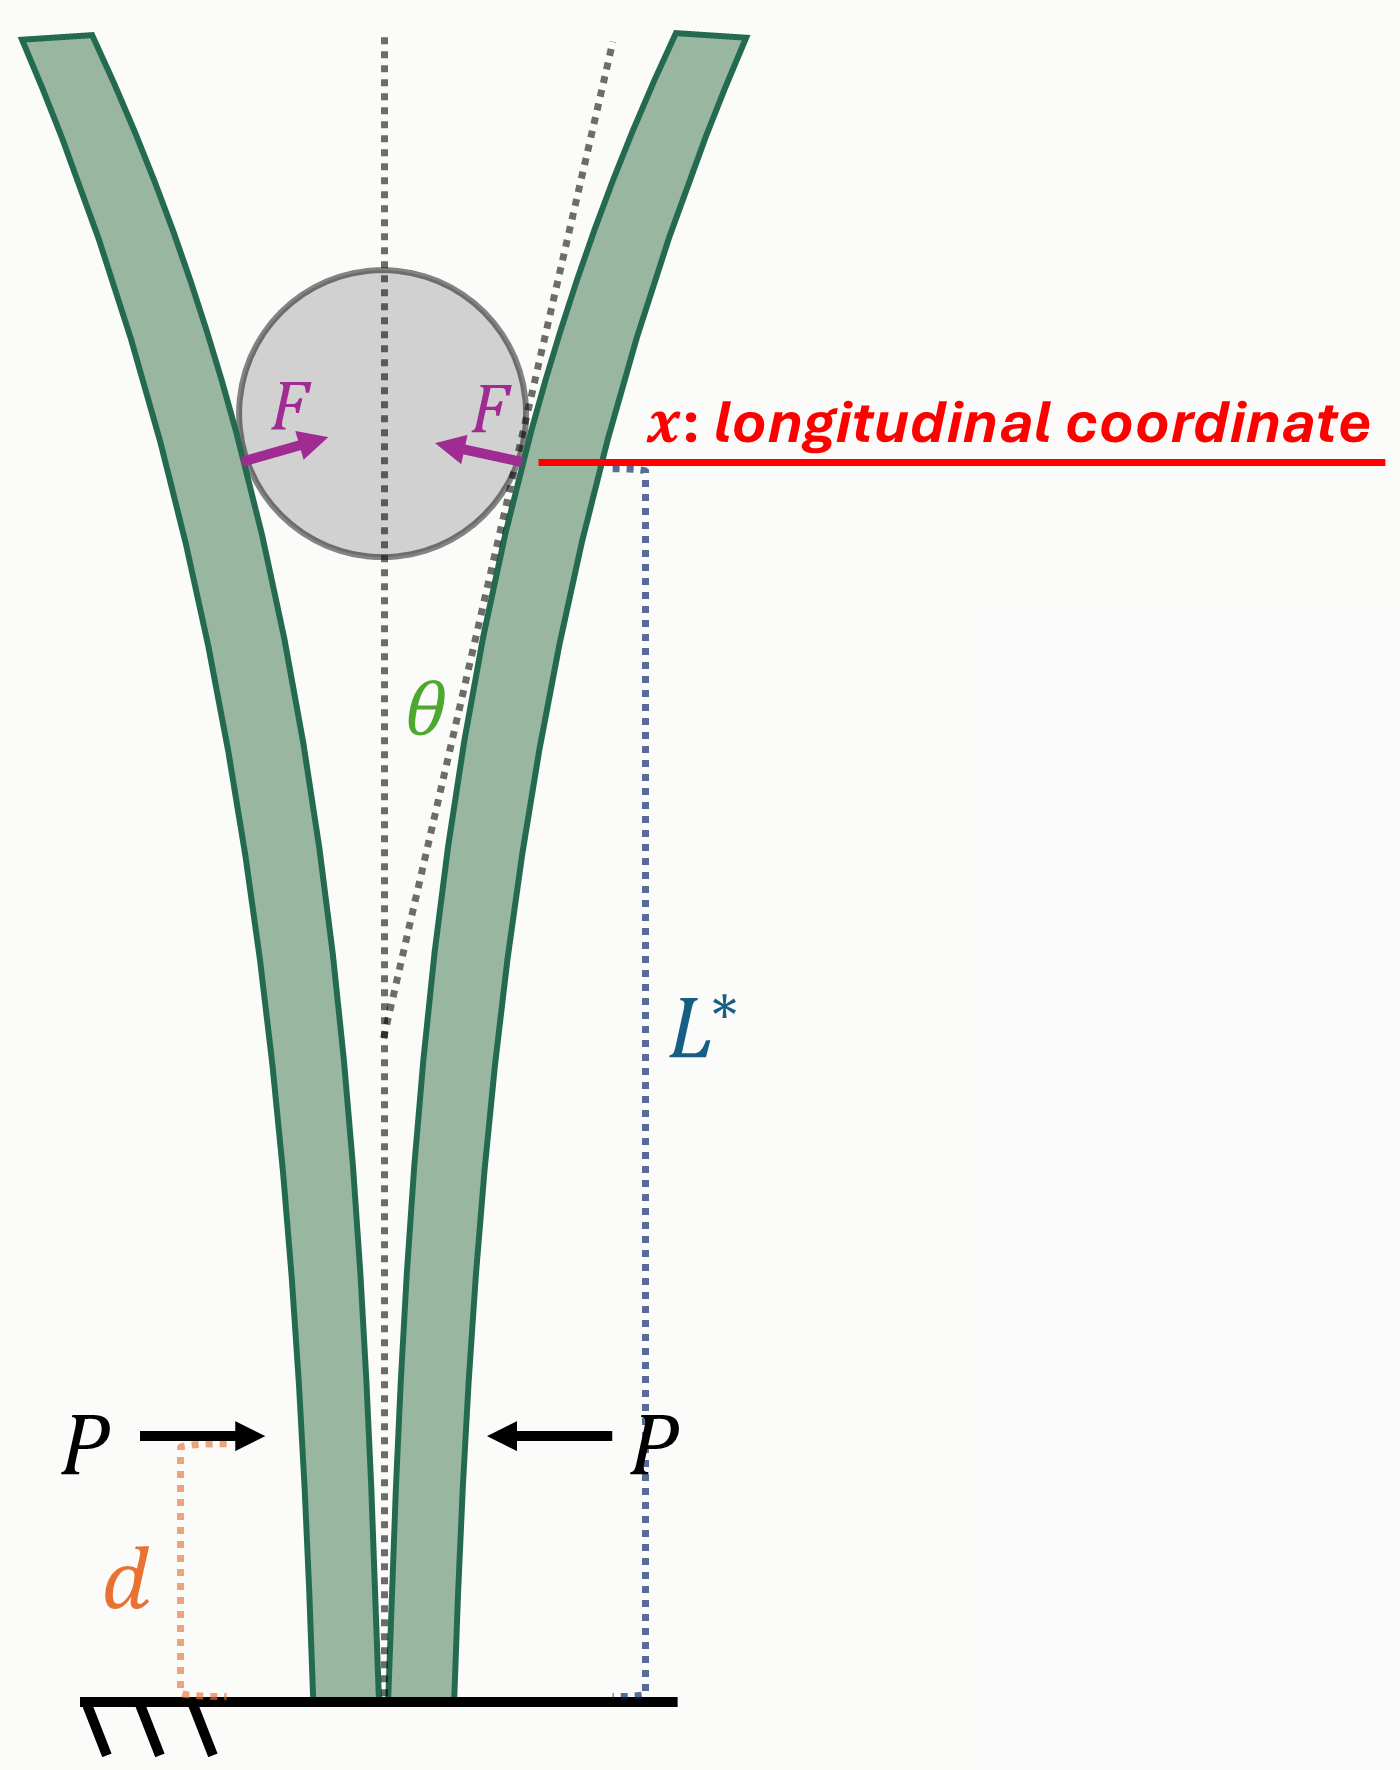
\includegraphics[width=0.55\columnwidth]{beam_diagram.png}
  \caption{Modelo das réguas como vigas em balanço: força de contato $F$ da bola, força extra $P$ aplicada à distância $d$ do engaste, inclinação $\theta$, coordenada longitudinal e comprimento $L^*=x_0$ entre o engaste e o ponto de contato.}
  \label{fig:beam}
\end{figure}

\subsection{Energia elástica, teorema de Castigliano e reciprocidade}

A energia de deformação armazenada em uma régua é
\begin{equation}
  U = \int_0^{x_0}\frac{M^2}{2EI}\,ds
  = \frac{1}{2EI}\int_0^{x_0}\Big[F\mac{x_0-s}-P\mac{d-s}\Big]^2 ds .
\end{equation}
O termo cruzado só contribui em $0<s<d$, onde $\int_0^d(x_0-s)(d-s)\,ds = (x_0-d)d^2/2+d^3/3$. Assim,
\begin{equation}
  U_0 = \frac{1}{2EI}\left[\frac{F^2x_0^3}{3} + \frac{P^2d^3}{3} - FPx_0d^2 + \frac{FPd^3}{3}\right].
  \label{eq:U0}
\end{equation}
Pelo teorema de Castigliano~\cite{castigliano}, o deslocamento do ponto de aplicação de uma força generalizada $Q_i$, na direção dela, é $\delta_i=\partial U/\partial Q_i$. Tomando $Q=(F,P)$, com $\delta_F=w(x_0)$ e $\delta_P=-w(d)$ (o deslocamento para dentro sob o atuador), a Eq.~\eqref{eq:U0} fornece a relação constitutiva completa do sistema,
\begin{equation}
  \begin{pmatrix}\delta_F\\ \delta_P\end{pmatrix}
  = \frac{1}{6EI}
  \begin{pmatrix} 2x_0^3 & -d^2(3x_0-d)\\ -d^2(3x_0-d) & 2d^3\end{pmatrix}
  \begin{pmatrix}F\\ P\end{pmatrix}.
  \label{eq:flex}
\end{equation}
A primeira linha reproduz a Eq.~\eqref{eq:defl}, o que verifica a integração de Macaulay. A matriz de flexibilidade é simétrica, como exige o teorema de reciprocidade de Maxwell--Betti~\cite{gere2009}: o deslocamento sob o atuador causado por uma força unitária no contato é igual ao deslocamento no contato causado por uma força unitária no atuador. Seu determinante,
\begin{equation}
  \det = \frac{4x_0^3d^3 - d^4(3x_0-d)^2}{36E^2I^2} = \frac{d^3(x_0-d)^2(4x_0-d)}{36E^2I^2},
\end{equation}
é positivo para $0<d<x_0$, de modo que $U_0$ é uma forma quadrática positiva definida, como deve ser para uma estrutura estável.

\subsection{Geometria de tangência e força de contato}

As réguas permanecem tangentes ao projétil. Se a régua está inclinada de $\theta$ no ponto de contato, o raio do projétil que chega ao contato faz o ângulo $\theta$ com a direção transversal (Fig.~\ref{fig:pinch}): o contato está deslocado de $r\cos\theta$ transversalmente e de $r\sin\theta$ ao longo do eixo em relação ao centro, e a força normal tem a componente axial $F\sin\theta$. A condição geométrica de contato, $w(x_0)=r\cos\theta$, dá a força de contato
\begin{equation}
  F = \frac{3EIr\cos\theta}{x_0^3} + \frac{Pd^2(3x_0-d)}{2x_0^3}.
  \label{eq:F_exact}
\end{equation}
A teoria de Euler--Bernoulli é linear na inclinação, e a correção $\cos\theta = 1-O(\theta^2)$ é da mesma ordem que os termos que ela despreza. De forma consistente, usamos daqui em diante
\begin{equation}
  F(x) = \frac{3EIr}{x^3} + \frac{Pd^2(3x-d)}{2x^3},
  \label{eq:F}
\end{equation}
escrita para uma posição genérica $x$ do contato; a geometria exata de tangência entra apenas como uma correção relativa de ordem $\mu_s^2/2$. O primeiro termo é a força devida apenas à bola; o segundo descreve como a força extra aumenta o momento fletor da régua.

\begin{figure}[t]
  \centering
  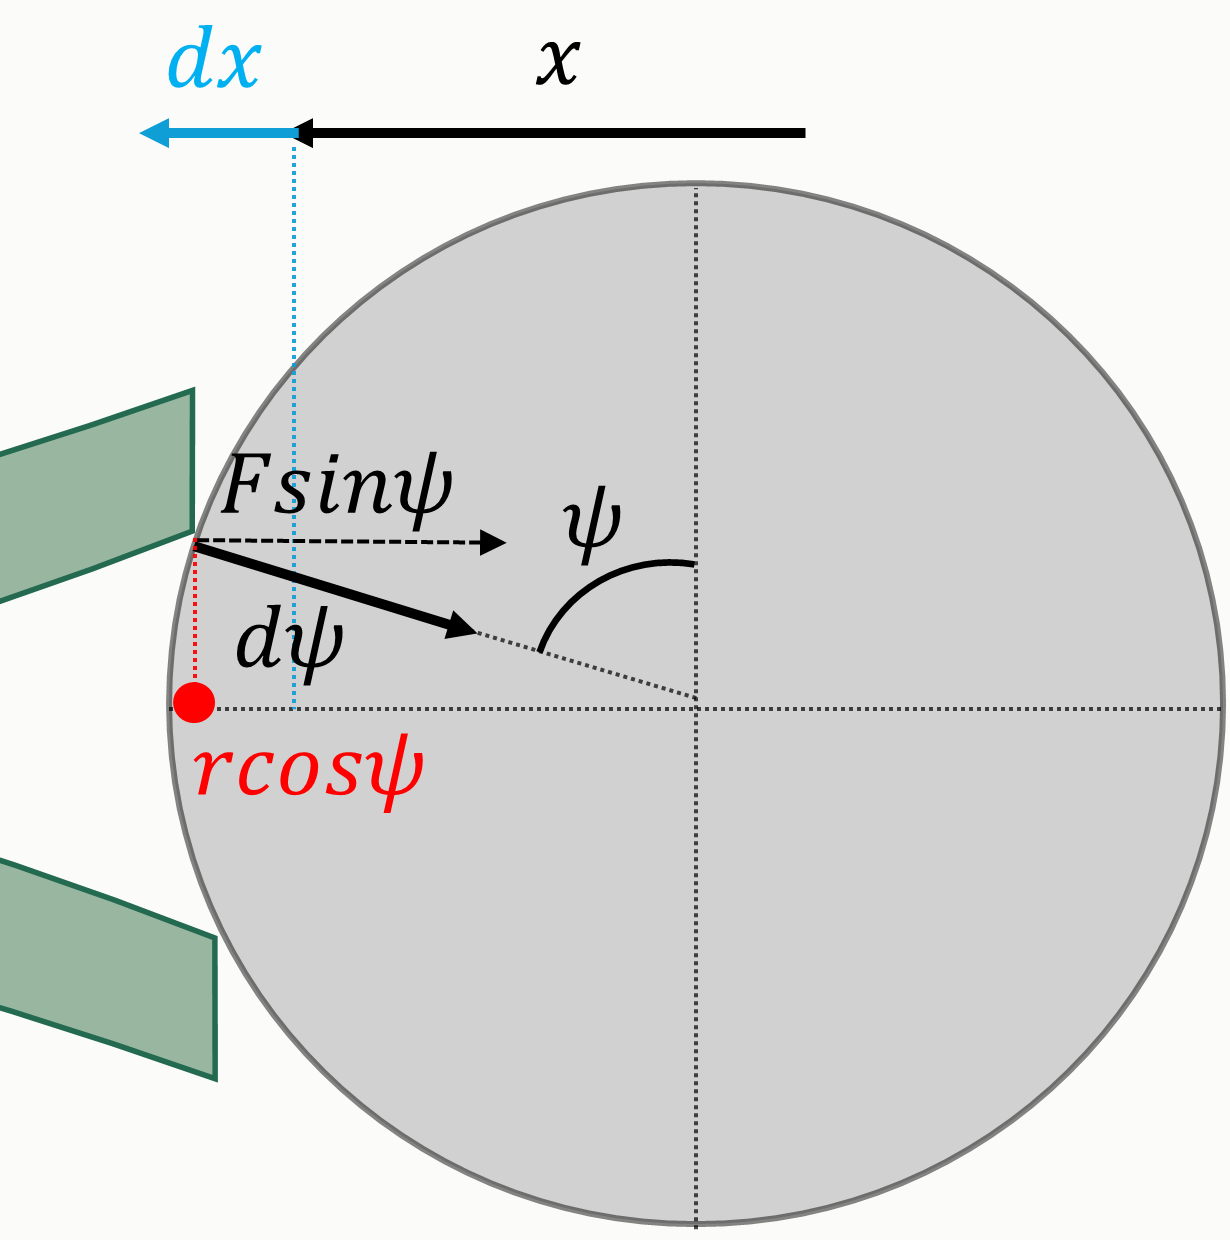
\includegraphics[width=0.6\columnwidth]{pinch_geometry.png}
  \caption{Geometria de tangência no contato: o raio que chega ao ponto de contato faz o ângulo $\psi=\theta$ com a direção transversal; o contato está deslocado de $r\cos\psi$ transversalmente, e $F\sin\psi$ é a componente axial da força normal, que empurra o projétil para fora.}
  \label{fig:pinch}
\end{figure}

\subsection{Atrito estático, condição de lançamento e zona de retenção}

No ponto de contato a régua está inclinada de $\theta$ em relação ao eixo do dispositivo (Fig.~\ref{fig:friction}). A componente axial da força de contato, $F\sin\theta$, empurra o projétil para fora e é equilibrada pelo atrito enquanto $F\sin\theta\le\mu_sF\cos\theta$. O projétil é liberado quando
\begin{equation}
  \tan\theta(x_0) = \mu_s .
  \label{eq:release}
\end{equation}
Com $\tan\theta\simeq\theta$ e as Eqs.~\eqref{eq:theta} e \eqref{eq:F} em $x=x_0$,
\begin{equation}
  \theta(x_0) = \frac{3r}{2x_0} + \frac{Pd^2(x_0-d)}{4EIx_0},
  \label{eq:theta0}
\end{equation}
e a força extra necessária ao lançamento é
\begin{equation}
  P^\ast = \frac{2EI\,(2\mu_sx_0-3r)}{d^2(x_0-d)} .
  \label{eq:P}
\end{equation}
A Eq.~\eqref{eq:P} resume o comportamento qualitativo. Um coeficiente de atrito estático maior exige uma força extra maior; uma inclinação inicial maior, ou um projétil maior, exige uma força menor. Três consequências merecem destaque.

\paragraph*{Zona de retenção e autoejeção.} Sem força extra, a inclinação no contato é $\theta_0=3r/2x_0$. O projétil só pode ser retido se $\theta_0<\mu_s$, isto é, na zona
\begin{equation}
  x_0 > x_{\min} = \frac{3r}{2\mu_s}.
  \label{eq:xmin}
\end{equation}
Se o projétil é inserido mais perto do engaste, $P^\ast\le0$ e ele é ejetado assim que é inserido (\emph{autoejeção}), efeito que observamos com os maiores projéteis. Com a geometria exata de tangência, $\theta_0$ é a raiz da equação transcendente $\theta_0=3r\cos\theta_0/2x_0$, e a fronteira da zona torna-se $x_{\min}=3r/\big(2\sqrt{1+\mu_s^2}\,\arctan\mu_s\big)$, que se reduz à Eq.~\eqref{eq:xmin} para $\mu_s\ll1$.

\paragraph*{Posição ótima do atuador.} Para $x_0$ fixo, $P^\ast\propto[d^2(x_0-d)]^{-1}$ diverge tanto quando o atuador se aproxima do engaste ($d\to0$, braço de alavanca nulo) quanto quando se aproxima do projétil ($d\to x_0$, momento fletor nulo no contato). A força necessária é mínima em
\begin{equation}
  d^\ast = \frac{2}{3}\,x_0, \qquad P^\ast_{\min} = \frac{27EI\,(2\mu_sx_0-3r)}{2x_0^3}.
  \label{eq:dopt}
\end{equation}

\paragraph*{Parâmetro de pré-carga.} Toda a dependência posterior em $P^\ast$ aparece através do número adimensional
\begin{equation}
  \beta \equiv \frac{P^\ast d^2}{4EI} = \frac{2\mu_sx_0-3r}{2(x_0-d)},
  \label{eq:beta}
\end{equation}
que independe de $EI$: a rigidez das réguas fixa a escala de forças, mas não a geometria do lançamento.

\begin{figure}[t]
  \centering
  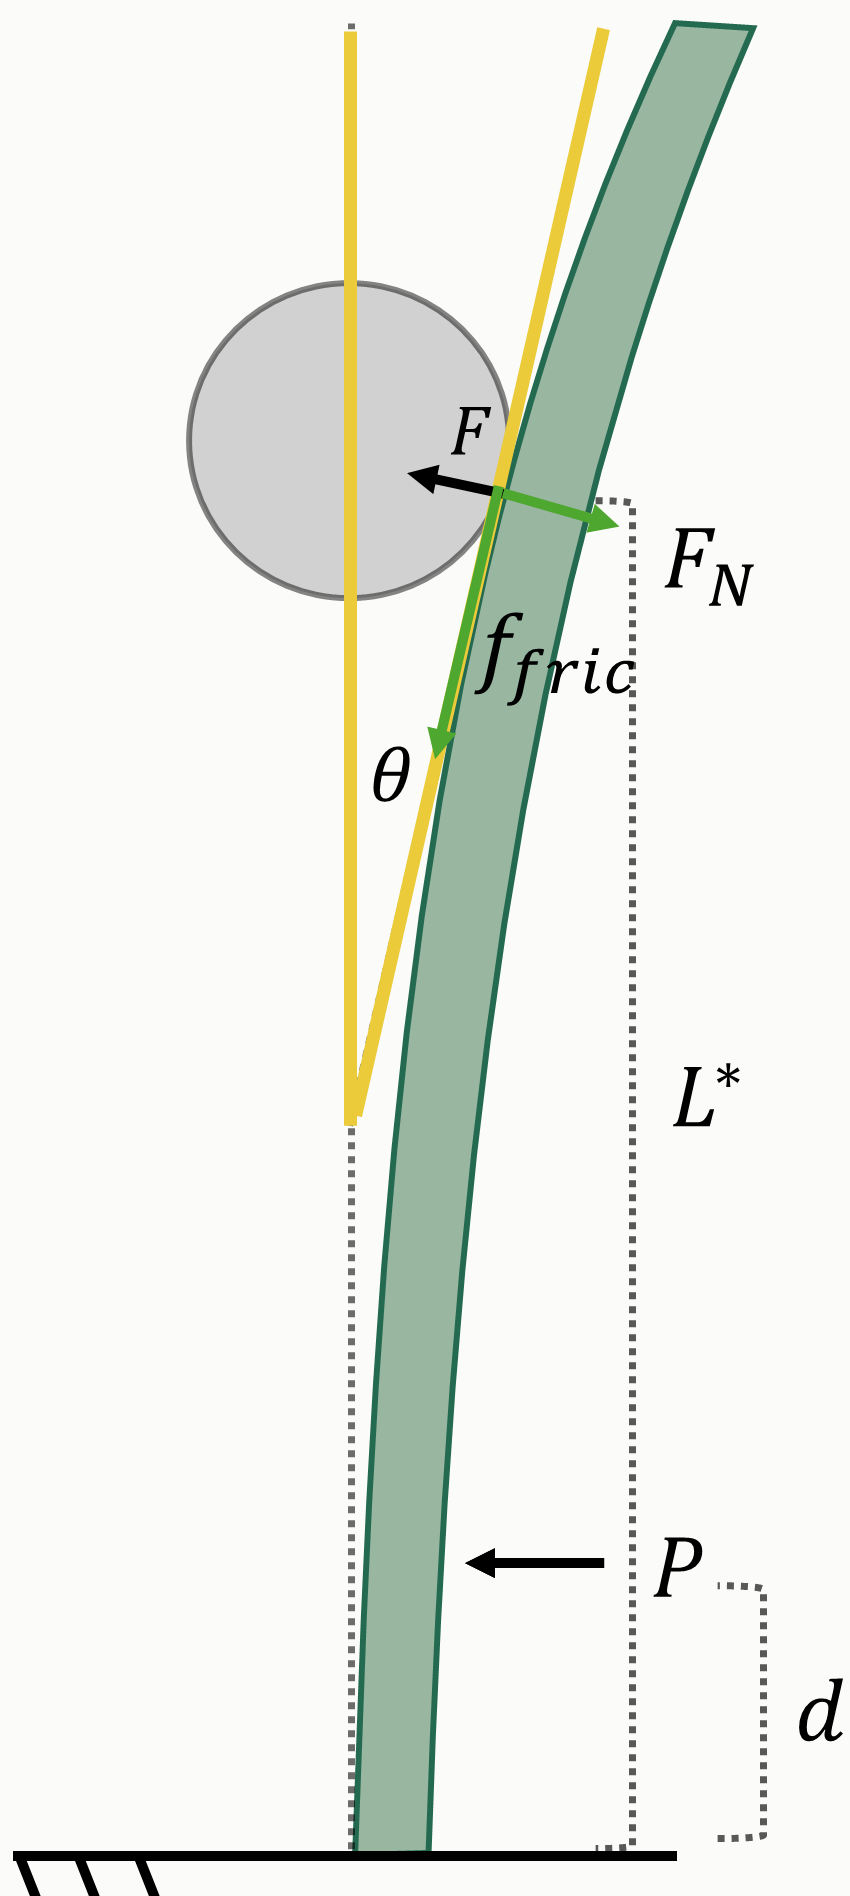
\includegraphics[width=0.36\columnwidth]{friction_diagram.png}
  \caption{Forças sobre a bola no ponto de contato: força normal $F_N$, atrito $f_{\mathrm{fric}}$ e o ângulo de contato $\theta$.}
  \label{fig:friction}
\end{figure}

\subsection{Dinâmica após a liberação}

Após a liberação, o projétil desliza de $x_0$ até a extremidade livre das réguas, em $x=L$. Tratamos as réguas como quase estáticas, de modo que as Eqs.~\eqref{eq:theta} e \eqref{eq:F} valem em cada posição $x$ com $P=P^\ast$ constante (as hastes dos atuadores se movem devagar em comparação com o projétil). Em cada régua, a componente axial da força de contato impulsiona o projétil, e o atrito cinético, de coeficiente $\mu_d$, se opõe a ele. As duas réguas aplicam torques de atrito iguais e opostos, de modo que o projétil não gira enquanto está comprimido. Os discos deslizam também sobre a base, com coeficiente $\mu_b$. Parte da energia liberada vai para o movimento das próprias réguas, que descrevemos por uma massa efetiva $m_r$. A equação de movimento do projétil é
\begin{multline}
  (m+m_r)\,\ddot x = 2F(x)\left[\sin\theta(x)-\mu_d\cos\theta(x)\right] \\
  - \mu_b\,mg\,\delta_{\mathrm{disco}},
  \label{eq:newton}
\end{multline}
com $\delta_{\mathrm{disco}}=1$ para discos e $0$ para esferas. Multiplicando por $\dot x$ e integrando de $x_0$ (repouso) a $L$, obtemos a primeira integral
\begin{multline}
  \tfrac12(m+m_r)v^2 = 2\int_{x_0}^{L}F(x)\left[\sin\theta(x)-\mu_d\cos\theta(x)\right]dx \\
  - \mu_b\,mg\,(L-x_0)\,\delta_{\mathrm{disco}} .
  \label{eq:energy}
\end{multline}
A energia elástica das réguas é liberada precisamente através do trabalho $\int F\sin\theta\,dx$ da componente axial da força de contato, de modo que ela não aparece como um termo separado: somá-la a esse trabalho a contaria duas vezes.

\paragraph*{Massa efetiva das réguas.} Pelo método de Rayleigh~\cite{rayleigh1877}, uma viga em balanço de massa $m_b$ que se move com a forma da sua deflexão estática sob carga na extremidade, $w\propto s^2(3L-s)$, tem energia cinética $\tfrac12(33/140)\,m_b\,\dot w_L^2$, onde $\dot w_L$ é a velocidade da extremidade. Para as duas réguas, $m_r\approx(33/70)\,m_b\approx0{,}5\,m_b$ quando o contato está próximo da extremidade; para contatos mais internos, o trecho reto além do contato aumenta essa fração. A massa efetiva entra no balanço de energia como uma inércia adicional do projétil.

\subsection{Velocidade de ejeção em forma fechada}

No limite de pequenas inclinações, $\sin\theta\simeq\theta$ e $\cos\theta\simeq1$, a integral da Eq.~\eqref{eq:energy} pode ser calculada exatamente. Usando a Eq.~\eqref{eq:beta}, a força e a inclinação ao longo do caminho tomam a forma compacta
\begin{equation}
  F(x) = \frac{EI}{x^3}\left(\mathcal A + 6\beta x\right),
  \qquad
  \theta(x) = \frac{\mathcal A}{2x} + \beta,
  \label{eq:Ftheta_compact}
\end{equation}
com
\begin{equation}
  \mathcal A = 3r-2\beta d = \frac{x_0\,(3r-2\mu_sd)}{x_0-d} .
\end{equation}
Pode-se verificar que $\theta(x_0)=\mu_s$, como exige a condição de liberação. O produto $F\theta$ é um polinômio em $1/x$, $F\theta=EI\big[\mathcal A^2/2x^4 + 4\mathcal A\beta/x^3 + 6\beta^2/x^2\big]$, e, definindo
\begin{equation}
  \Delta_k \equiv x_0^{-k} - L^{-k},
\end{equation}
a velocidade de ejeção é
\begin{widetext}
\begin{equation}
  v^2 = \frac{4EI}{m+m_r}\left[\frac{\mathcal A^2}{6}\,\Delta_3 + 2\mathcal A\beta\,\Delta_2 + 6\beta^2\,\Delta_1
  - \mu_d\left(\frac{\mathcal A}{2}\,\Delta_2 + 6\beta\,\Delta_1\right)\right]
  - \frac{2\mu_b\,mg\,(L-x_0)}{m+m_r}\,\delta_{\mathrm{disco}} .
  \label{eq:vclosed}
\end{equation}
\end{widetext}
A Eq.~\eqref{eq:vclosed} torna explícitas as dependências do problema. (i)~Para um projétil esférico, $v\propto\sqrt{EI/(m+m_r)}$: réguas mais rígidas lançam mais depressa, e a massa entra apenas pela inércia total. (ii)~Como $\beta$ e $\mathcal A$ dependem de $r$, $x_0$, $d$ e $\mu_s$, mas não de $EI$, a forma das curvas $v(r)$, $v(x_0)$ e $v(d)$ das esferas é independente da rigidez, que fixa apenas sua escala. (iii)~Quando $x_0\to L$, todos os $\Delta_k\to0$ e $v\to0$. (iv)~Quando $d\to x_0$, $\beta$ cresce sem limite: a força extra, e com ela a energia armazenada, aumenta à medida que os atuadores se aproximam do projétil.

\paragraph*{Comprimento ótimo das réguas.} O projétil só é acelerado enquanto $\theta(x)>\mu_d$. Como $\theta(x)$ decresce monotonamente de $\mu_s$ até $\beta$, se $\beta<\mu_d$ existe uma posição
\begin{equation}
  x^\dagger = \frac{\mathcal A}{2(\mu_d-\beta)}
  \label{eq:xdagger}
\end{equation}
além da qual o atrito cinético supera o impulso das réguas e o projétil desacelera. Réguas mais longas que $x^\dagger$ não aumentam a velocidade de ejeção, e a velocidade máxima é atingida em $L=x^\dagger$.

%=====================================================================
\section{Resultados e discussão}
\label{sec:results}
%=====================================================================

As medidas foram ajustadas com a Eq.~\eqref{eq:energy}, avaliada numericamente sem a aproximação de pequenas inclinações (Figs.~\ref{fig:v_r}--\ref{fig:v_m}). O ajuste usa a rigidez da régua~1, as razões de rigidez $k_{2,3}=EI_{2,3}/EI_1$, os coeficientes de atrito $\mu_s$, $\mu_d$ e $\mu_b$, a massa efetiva $m_r$ e os valores de $x_0$ e $d$ mantidos fixos em cada série. Sobre os 120 pontos, o desvio quadrático médio é de \SI{0.15}{m/s}.

Uma única família de réguas, contudo, não descreve as quatro séries. As velocidades absolutas das séries de posição inicial e de massa são muito menores que as das outras duas (compare as Figs.~\ref{fig:v_r} e \ref{fig:v_x0} em valores semelhantes de $x_0$). O ajuste exige, portanto, uma escala de rigidez independente para cada série, e essas escalas cobrem um fator de cerca de 15. Isso sugere que as réguas, ou o curso dos atuadores, diferiram entre as séries. Dentro de cada série as tendências são reproduzidas, mas os valores absolutos de $EI$, $\mu_s$, $\mu_d$ e os valores fixos de $x_0$ e $d$ são fortemente correlacionados e não são determinados individualmente, como antecipa a propriedade~(ii) da Eq.~\eqref{eq:vclosed}. Os parâmetros bem determinados estão na Tabela~\ref{tab:fit7}.

\begin{table}[b]
  \caption{Parâmetros da Eq.~\eqref{eq:energy} bem determinados pelo ajuste (incertezas: um desvio padrão).}
  \label{tab:fit7}
  \begin{ruledtabular}
  \begin{tabular}{lc}
    Parâmetro & Valor ajustado \\
    \midrule
    Razão de rigidez $EI_2/EI_1$ & $0{,}53\pm0{,}02$ \\
    Razão de rigidez $EI_3/EI_1$ & $0{,}49\pm0{,}02$ \\
    Atrito disco--base $\mu_b$ & $0{,}20\pm0{,}08$ \\
    Massa efetiva das réguas $m_r$ (g) & $46\pm28$ \\
    $x_0$ na série de $d$ (cm) & $21\pm5$ \\
  \end{tabular}
  \end{ruledtabular}
\end{table}

\paragraph*{Esferas e discos.} As esferas são ligeiramente mais rápidas que discos de mesma massa (Fig.~\ref{fig:v_m}). No modelo, isso se deve ao atrito dos discos com a base, $\mu_b\approx0{,}2$. Na série de raio, os discos são mais leves que as esferas (\SI{28.7}{g} contra \SI{33.8}{g}), o que compensa o atrito com a base, e as duas formas atingem quase a mesma velocidade (Fig.~\ref{fig:v_r}). Fora isso, as duas formas se comportam da mesma maneira, o que é consistente com a ausência de rotação enquanto o projétil está comprimido: a grandeza relevante é a seção circular do projétil no plano das réguas.

\paragraph*{Raio.} A velocidade de ejeção diminui com o raio do projétil (Fig.~\ref{fig:v_r}). Esse resultado contraintuitivo é capturado pelo modelo: projéteis maiores precisam de uma força extra menor para vencer o atrito estático, Eq.~\eqref{eq:P}, e por isso menos energia está armazenada no momento da liberação. No limite $r\to2\mu_sx_0/3$, a pré-carga $\beta$ se anula e o projétil atinge a fronteira da zona de retenção, Eq.~\eqref{eq:xmin}.

\begin{figure}[t]
  \centering
  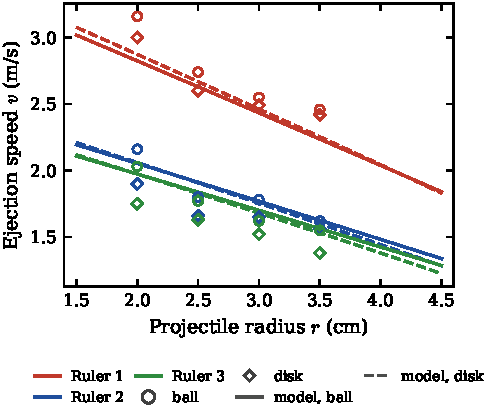
\includegraphics[width=\columnwidth]{v_vs_r_fit.pdf}
  \caption{Velocidade de ejeção em função do raio $r$ do projétil (metade dos diâmetros da Tabela~\ref{tab:projectiles}). Linhas: ajuste da Eq.~\eqref{eq:energy} para esferas (contínua) e discos (tracejada); marcadores: experimento.}
  \label{fig:v_r}
\end{figure}

\paragraph*{Posição da força extra.} A velocidade aumenta com $d$ (Fig.~\ref{fig:v_d}). Pela Eq.~\eqref{eq:beta}, a pré-carga $\beta\propto(x_0-d)^{-1}$ cresce à medida que os atuadores se aproximam do projétil, o que eleva a força de contato e a inclinação ao longo de todo o caminho, Eq.~\eqref{eq:Ftheta_compact}. Fisicamente, para vencer o atrito estático com o atuador próximo ao contato, é preciso fletir muito a régua, e essa energia adicional é devolvida ao projétil.

\begin{figure}[t]
  \centering
  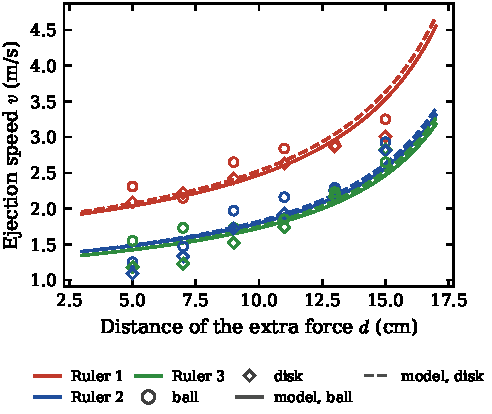
\includegraphics[width=\columnwidth]{v_vs_d_fit.pdf}
  \caption{Velocidade de ejeção em função da distância $d$ da força extra. Linhas: ajuste da Eq.~\eqref{eq:energy} para esferas (contínua) e discos (tracejada); marcadores: experimento.}
  \label{fig:v_d}
\end{figure}

\paragraph*{Posição inicial.} A velocidade diminui quando o projétil parte mais longe do engaste (Fig.~\ref{fig:v_x0}). A força de contato decresce como $x_0^{-3}$ e o caminho até a extremidade das réguas fica mais curto, de modo que $v\to0$ quando $x_0\to L$, como mostra a Eq.~\eqref{eq:vclosed}. Para discos, o modelo prevê que o atrito com a base os detém antes de $x_0\approx\SI{27}{cm}$, ligeiramente além do maior $x_0$ medido.

\begin{figure}[t]
  \centering
  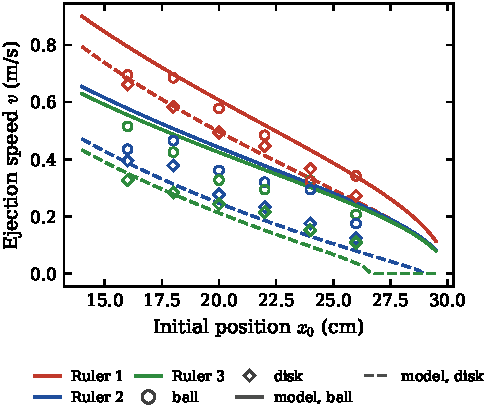
\includegraphics[width=\columnwidth]{v_vs_x0_fit.pdf}
  \caption{Velocidade de ejeção em função da posição inicial $x_0$. Linhas: ajuste da Eq.~\eqref{eq:energy} para esferas (contínua) e discos (tracejada); marcadores: experimento.}
  \label{fig:v_x0}
\end{figure}

\paragraph*{Massa.} Projéteis mais pesados são mais lentos (Fig.~\ref{fig:v_m}), mas a velocidade medida cai aproximadamente como $m^{-1/3}$, mais devagar que o $m^{-1/2}$ esperado se toda a energia fosse para o projétil. A massa efetiva das réguas explica esse comportamento: com $v\propto(m+m_r)^{-1/2}$, a dependência em $m$ é mais fraca quando $m$ não é muito maior que $m_r$. O valor ajustado, $m_r=(46\pm28)$~g, corresponde, pelo argumento de Rayleigh, a réguas de algumas dezenas de gramas, plausível para réguas comuns de \SI{30}{cm}.

\begin{figure}[t]
  \centering
  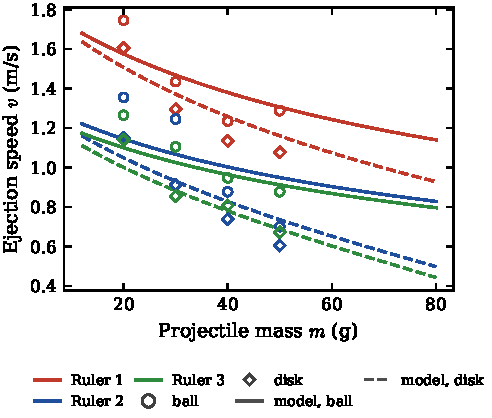
\includegraphics[width=\columnwidth]{v_vs_m_fit.pdf}
  \caption{Velocidade de ejeção em função da massa $m$ do projétil, com diâmetro de \SI{4}{cm}. Linhas: ajuste da Eq.~\eqref{eq:energy} para esferas (contínua) e discos (tracejada); marcadores: experimento.}
  \label{fig:v_m}
\end{figure}

Para todos os parâmetros, a régua~1 produz velocidades sistematicamente maiores que as réguas~2 e 3, o que é consistente com $v\propto\sqrt{EI}$ e com as razões de rigidez ajustadas, próximas de um meio.

%=====================================================================
\section{Conclusão}
\label{sec:conclusion}
%=====================================================================

O canhão de réguas armazena energia elástica em duas vigas em balanço e a libera quando a força extra sobre as réguas eleva a inclinação no contato além do ângulo de atrito. Uma formulação de Macaulay da viga de Euler--Bernoulli, verificada pelo teorema de Castigliano e pela simetria de Maxwell--Betti da matriz de flexibilidade, fornece a força de contato e a força extra necessária ao lançamento. Esta define uma zona de retenção, cuja fronteira explica a autoejeção dos projéteis grandes, e uma posição ótima do atuador em dois terços da distância ao projétil. Escrevendo o balanço de energia como o trabalho das forças de contato, sem contar a energia armazenada duas vezes, obtivemos a velocidade de ejeção em forma fechada, com escala $\sqrt{EI/(m+m_r)}$ e forma independente da rigidez. O modelo reproduz as tendências medidas com o raio, a posição da força extra, a posição inicial e a massa, e explica as esferas mais rápidas (atrito dos discos com a base) e a fraca dependência com a massa (inércia das réguas). Ele não descreve todas as séries com uma única família de réguas: as séries diferem em velocidade absoluta mais do que o modelo permite, o que aponta para diferenças entre as réguas ou entre os ajustes dos atuadores de uma série para outra.

\bibliography{references}

\end{document}
